%
% ======================================================================
% INFORMATION
%
% This document may be used as a template for SMiP presentations in 
% LaTeX Beamer, based on Martin Schnuerch's Markdown template and SMiP's 
% PowerPoint template. 
% You can further customize the presentation's theme by changing the underlying 
% "beamer...themesmipstyle.sty" documents. There is no warranty whatsoever 
% that the document has been coded in best/appropriate LaTeX style.
%
% To insert your university's logo, store the file in the "subfiles" folder
% and replace "mannheim.pdf" in line 34 with the correct name (you may also want
% to adjust the "width" argument in case the logo appears too large/small).
%
% I hope you enjoy the template and I am grateful for questions, comments, or
% suggestions: susanne.frick@uni-mannheim.de 
%
% ======================================================================
%
% Update: Template x.personalized
% I customized Susanne Frick's template to fit my needs and added my avatar,
% and a few custom features that I use often. All praise goes to her, but if
% any questions arise about my customizations, feel free to contact me:
% bissantz[at]uni-landau.de
%
% ======================================================================
%

%------------------ preamble -----------------------------------

\documentclass[10pt]{beamer}
\mode<presentation>{
	\usetheme{smipstyle}
}

%------------------ title and author name ----------------------

\title[A few words about myself]{A few words about myself}

\titlegraphic{
\includegraphics[width=4cm]{subfiles/landau.eps}}
\author{Steven Marcel Bißantz}
\institute{University of Koblenz$\cdot$Landau}
\date[SMiP Fall Reatreat 2022]{Fall Retreat 2022, November 25 -- 26, Ludwigshafen}

%------------------ document content ---------------------------

\begin{document}

	%-------------- titlepage

	\begin{frame}
		\titlepage 
	\end{frame}
	
	%-------------- outline

	%\begin{frame}
		%\frametitle{Outline} 
		%\tableofcontents
	%\end{frame}
	
	%-------------- content

	\begin{frame}{Curriculum Vitae}
		\begin{columns}
			\begin{column}{0.6\textwidth}
				{\large Education}\\[2ex]
				\begin{description}
					\item[since 2022] SMiP Associate\\{\tiny (University of Koblenz$\cdot$Landau) }
					\item[since 2021] Ph.D. Candidate, Psychology\\ {\tiny(University of Koblenz$\cdot$Landau)}
					\item[2019-2021] M.A., Social Sciences\\{\tiny(University of Koblenz$\cdot$Landau)}
					\item[2014-2018] B.A., Sociology\\ {\tiny(University of Mannheim)}
				\end{description}
			\end{column}
			\begin{column}{0.4\textwidth}
				\visible<2>{
				\begin{figure}
					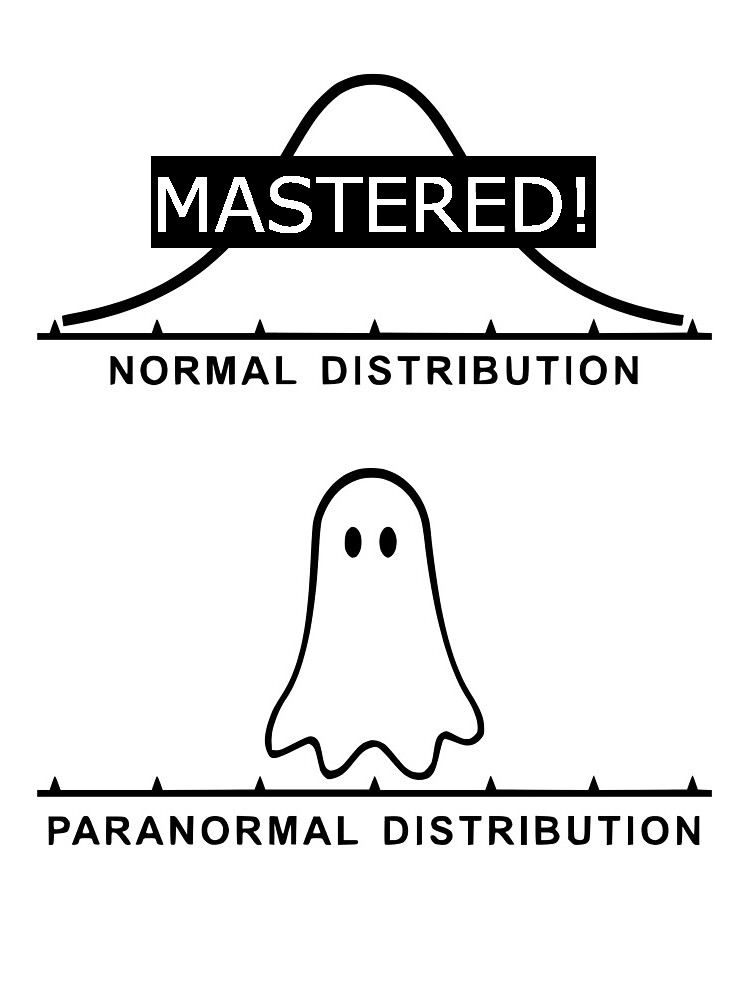
\includegraphics[width=4cm, trim = 0mm 10mm 0mm 0mm]{subfiles/paranormal_2.png}
					\caption{Possibilities for further research and new developments}
				\end{figure}
				}
			\end{column}
		\end{columns}
	\end{frame}

	\begin{frame}{Research \& Personal Interests}
		\begin{columns}
			\begin{column}{0.6\textwidth}
				{\large Research interests}\\[2ex]
				\begin{description}
					\item[primary] Meta-research\\[2ex]
					\item[primary] Statistical modeling\\[2ex]
					\item[primary] Statistical computing\\[2ex]
					\item[secondary] Do-calculus\\[2ex]
					\item[secondary] Missing data\\[2ex]
				\end{description}
			\end{column}
			\begin{column}{0.4\textwidth}
				\visible<2>{
				\begin{figure}
					\frame{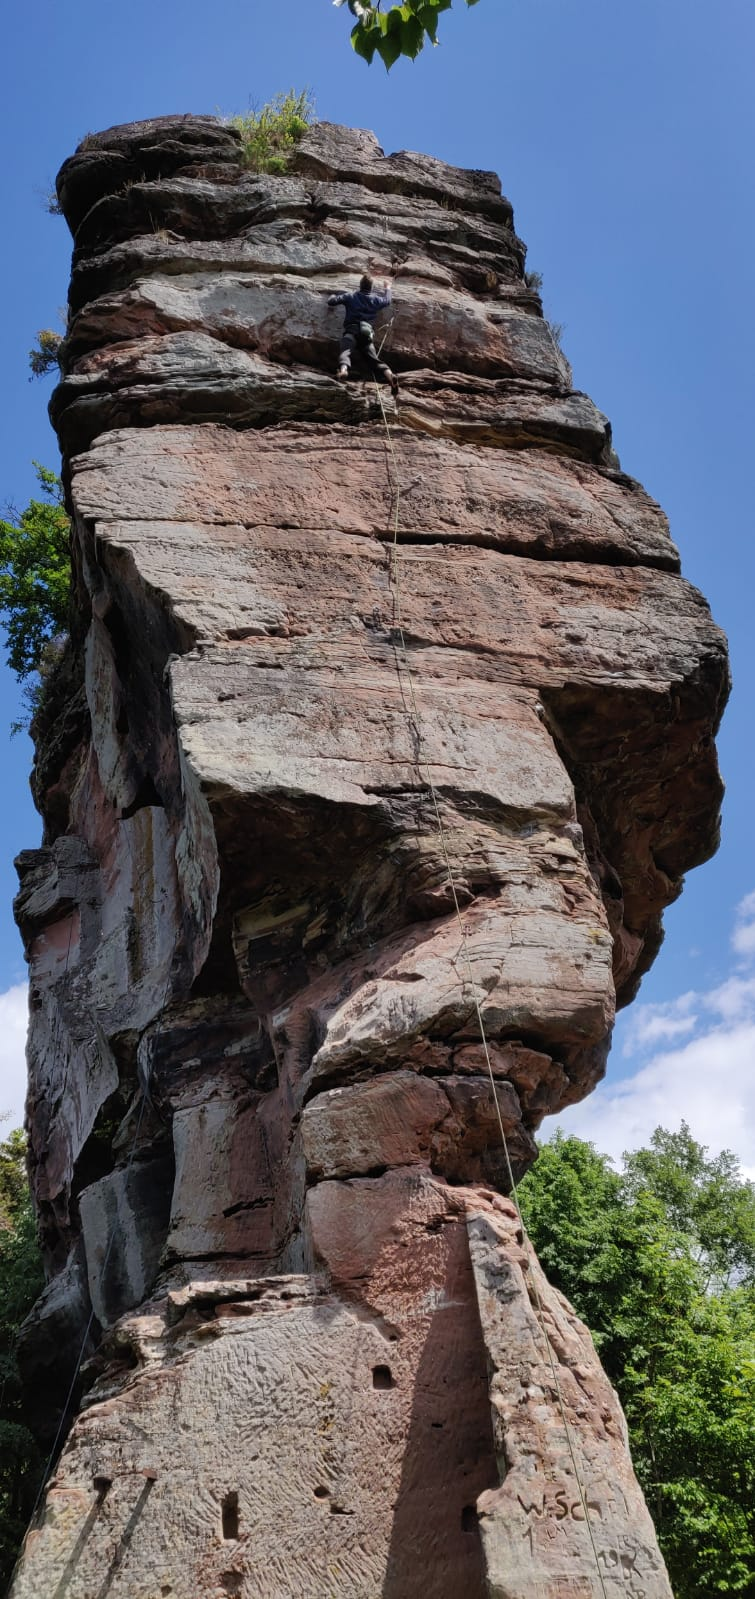
\includegraphics[height=5cm, clip=true, trim = 0mm 200mm 0mm 0mm]{subfiles/climbing.jpg}}
					\caption{Personal Interest -- climbing in the Alsatian sandstone}
					\end{figure}
				}
			\end{column}
		\end{columns}
	\end{frame}

	\begin{frame}{Measurement \& Replicability}
		\begin{multicols}{2}
			\emph{Research question}: What is the role of item-based
			measurement in the replicability of empirical findings?\\[4ex]
			\begin{figure}
				
\includegraphics[scale=.5]{subfiles/metarep.jpg}
			\end{figure}
		\end{multicols}
		\vspace{1ex}
		\visible<2,3,4>	{
			\emph{Focus}: Direct replications\\[2ex]
		}
		\visible<3,4>	{
			\begin{figure}
				\centering
				\begin{tikzpicture}[
					roundnode/.style={circle, draw=smipblue!60, fill=green!5, very thick, minimum size=7mm},
					squarednode/.style={rectangle, draw=smipblue!60, fill=red!5, very thick, minimum size=5mm},
					]
					%Nodes
					\node[squarednode]      (adhoc)			    			{Ad-hoc scales};
					\node[squarednode]      (modified)       [below=of adhoc] {Modified scales};
					\node[squarednode]      (estimate)       [right=of adhoc] {Effect-size estimates};
					\node[squarednode]      (heterogeneity)  [below=of estimate, right=of modified] {Effect-size heterogeneity};
					%Lines
					\draw[->] (adhoc.east) -- (estimate.west);
					\draw[->] (adhoc.east) -- (heterogeneity.west);
					\draw[->] (modified.east) -- (heterogeneity.west);
					\draw[->] (modified.east) -- (estimate.west);
				\end{tikzpicture}
			\end{figure}
			}
			\vspace{2ex}
			\visible<4>	{
				\emph{Scope}: 3 projects (experiment, simulation, [pending])
			}	
	\end{frame}

	%--------------- Aacknowledgments 

	\begin{frame}{Acknowledgments}
		\vspace{1cm}
		\begin{columns} 
			\begin{column}{.48\textwidth} 
				\begin{figure}[p]
					
\includegraphics[width=150px]{subfiles/logo_full.eps}
				\end{figure}
			\end{column}
			\begin{column}{.48\textwidth} 
				\begin{center}
					\footnotesize{This research was funded by the Deutsche
					Forschungsgemeinschaft (DFG), grant 2277, Research Training
				Group ``Statistical Modeling in Psychology" (SMiP)}
				\end{center}
			\end{column}
		\end{columns}
	\end{frame}
\end{document}

